\documentclass{article}\usepackage[]{graphicx}\usepackage[]{color}
%% maxwidth is the original width if it is less than linewidth
%% otherwise use linewidth (to make sure the graphics do not exceed the margin)
\makeatletter
\def\maxwidth{ %
  \ifdim\Gin@nat@width>\linewidth
    \linewidth
  \else
    \Gin@nat@width
  \fi
}
\makeatother

\definecolor{fgcolor}{rgb}{0.345, 0.345, 0.345}
\newcommand{\hlnum}[1]{\textcolor[rgb]{0.686,0.059,0.569}{#1}}%
\newcommand{\hlstr}[1]{\textcolor[rgb]{0.192,0.494,0.8}{#1}}%
\newcommand{\hlcom}[1]{\textcolor[rgb]{0.678,0.584,0.686}{\textit{#1}}}%
\newcommand{\hlopt}[1]{\textcolor[rgb]{0,0,0}{#1}}%
\newcommand{\hlstd}[1]{\textcolor[rgb]{0.345,0.345,0.345}{#1}}%
\newcommand{\hlkwa}[1]{\textcolor[rgb]{0.161,0.373,0.58}{\textbf{#1}}}%
\newcommand{\hlkwb}[1]{\textcolor[rgb]{0.69,0.353,0.396}{#1}}%
\newcommand{\hlkwc}[1]{\textcolor[rgb]{0.333,0.667,0.333}{#1}}%
\newcommand{\hlkwd}[1]{\textcolor[rgb]{0.737,0.353,0.396}{\textbf{#1}}}%

\usepackage{framed}
\makeatletter
\newenvironment{kframe}{%
 \def\at@end@of@kframe{}%
 \ifinner\ifhmode%
  \def\at@end@of@kframe{\end{minipage}}%
  \begin{minipage}{\columnwidth}%
 \fi\fi%
 \def\FrameCommand##1{\hskip\@totalleftmargin \hskip-\fboxsep
 \colorbox{shadecolor}{##1}\hskip-\fboxsep
     % There is no \\@totalrightmargin, so:
     \hskip-\linewidth \hskip-\@totalleftmargin \hskip\columnwidth}%
 \MakeFramed {\advance\hsize-\width
   \@totalleftmargin\z@ \linewidth\hsize
   \@setminipage}}%
 {\par\unskip\endMakeFramed%
 \at@end@of@kframe}
\makeatother

\definecolor{shadecolor}{rgb}{.97, .97, .97}
\definecolor{messagecolor}{rgb}{0, 0, 0}
\definecolor{warningcolor}{rgb}{1, 0, 1}
\definecolor{errorcolor}{rgb}{1, 0, 0}
\newenvironment{knitrout}{}{} % an empty environment to be redefined in TeX

\usepackage{alltt}
\usepackage[utf8]{inputenc}
\usepackage[hmargin=2cm,vmargin=1.5cm,bmargin=1.5cm]{geometry}
\title{Análise estatística de dados com objetivo de identificar clientes propensos a cancelar produtos de um banco}
\author{Daniel V. F. Falbel}
\date{16 de Novembro de 2014}
\IfFileExists{upquote.sty}{\usepackage{upquote}}{}
\begin{document}
\maketitle

\section*{Resumo}

Para auxiliar um banco na criação de ações publicitárias para retenção de clientes que possuem um certo cartão de crédito, este trabalho apresenta uma análise estatística que permite a identificação dos clientes mais propensos a cancelar o produto. Através de uma análise exploratória dos dados, foi identificado que a evolução dos saldos do cliente (credor, devedor ou da poupança) além do seu salário eram variáveis importantes para a explicação do tempo até o cancelamento do cartão de crédito.

\section{Descrição do problema}

Um banco deseja fazer ações de marketing para reter os seus clientes, evitar que eles cancelem seus produtos. Para poder fazer ações mais acertivas, o banco deseja saber qual é o perfil dos clientes com maior propensão a cancelar um certo cartão de crédito.

As variáveis que podem ajudar na identificação dos perfis estão listadas abaixo: 

\begin{itemize}
  \item sexo: M-masculino; F-feminino
  \item modulo: Segmentação de clientes; valores mais baixos representam clientes com menor renda ou investimento, valores mais altos representam clientes mais interessantes para a instituição
  \item cheque: Classificação da conta corrente; quanto maior o valor, mais "especial" o cliente
  \item evolcredor: Evolução do saldo credor médio trimestral (A: aumentou, D: diminuiu, M: manteve)
  \item evoldevedor: Evolução do saldo devedor médio trimestral (A: aumentou, D: diminuiu, M: manteve)
  \item evolpoup:  do saldo da poupança trimestral (A: aumentou, D: diminuiu, M: manteve)
  \item idade: idade em anos
  \item salario: está categorizado em 10 categorias (quanto maior, maior o salário)
  \item cartaocancel: Cancelamento do cartão de credito pelo banco 0 - não cancelou; 1 - cancelou
  \item bancsal: 0: não recebe salário pelo banco; 1: recebe salário pelo banco
  \item tempo: Tempo de permanência com um determinado produto, em meses
  \item status: 1: tempo refere-se ao tempo da contratação até o cancelamento do produto; 0: tempo da contratação até término de acompanhamento sem cancelamento (censura)
\end{itemize}

\section{Análise Descritiva}



Para verificar se existem possíveis inconsistências nos dados, foi feita uma análise exploratória. Além disso, podemos já ter uma ideia do que pode influencia no tempo até o cancelamento do cartão de crédito. 

\begin{figure}
\centering
\begin{knitrout}
\definecolor{shadecolor}{rgb}{0.969, 0.969, 0.969}\color{fgcolor}
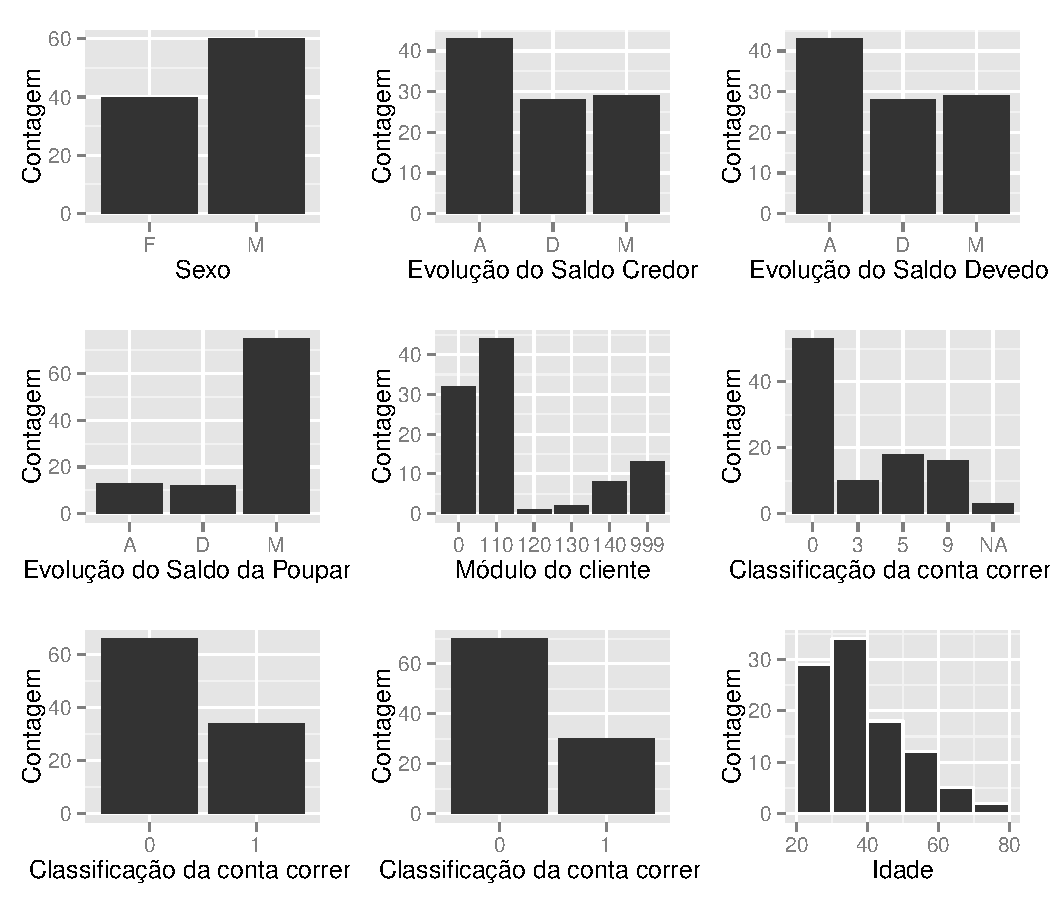
\includegraphics[width=\maxwidth]{figure/unnamed-chunk-2} 

\end{knitrout}
\caption{(i) quantidade de clientes em cada categoria da variável sexo, (ii) quantidade de clientes em cada categoria de evolução do saldo credor, (iii) quantidade de clientes em cada categoria de evolução do saldo devedor, (iv) quantidade de clientes em cada categoria de evolução do saldo da poupança, (v) quantidade de clientes em cada módulo (segmento) criado pelo banco, (vi) quantidade de clientes em  cada classificação da conta corrente, (vii) quantidade de clientes que cancelaram o cartão (1), (viii) quantidade de clientes que recebem o salário por meio do banco, (ix) histograma da idade dos clientes}
\end{figure}

Pelos gráficos da figura 1, podemos observar que 60\% dos clientes são do sexo masculino. A maior parte dos clientes teve um aumento do saldo credor e do saldo devedor. Também podemos analisar que a maior parte dos clientes manteve estável o saldo da poupança. Observamos que a maior parte dos clienes estão no segmento 110 do módulo, e que cerca de 50\% dos cliente estão na classificação 0 da conta corrente. Note que no gráfico (vi) existe a ocorrência de uma observação ausente, isto é, não temos a informação de que tipo de conta o cliente ppossui.

\begin{figure}[t!]

\centering
\begin{knitrout}
\definecolor{shadecolor}{rgb}{0.969, 0.969, 0.969}\color{fgcolor}
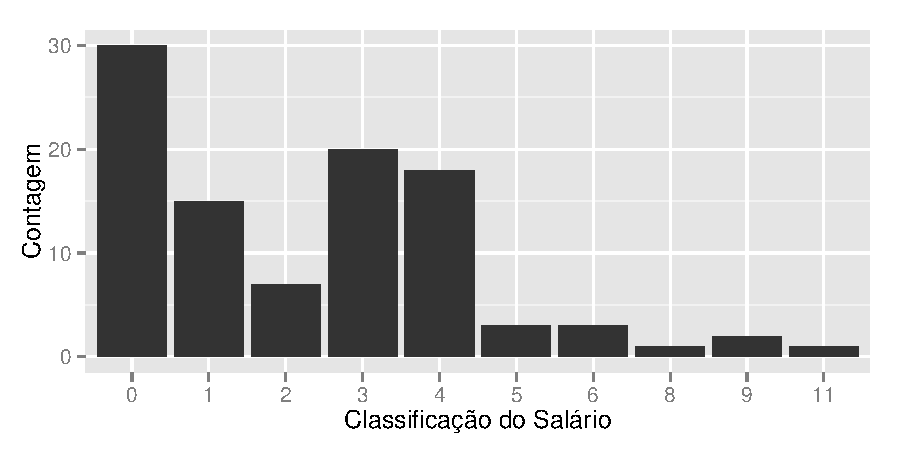
\includegraphics[width=\maxwidth]{figure/unnamed-chunk-3} 

\end{knitrout}
\caption{Quantidade de clientes em cada classificação do salário}
\end{figure}

Pela figura 2 observamos que cerca de 30\% dos clientes ganham até R\$300,00, em seguida as categorias com mais indivíduos são a 3 e a 4 que contém pessoas que ganham de R\$501,00 a R\$1500,00.

\begin{figure}[t!]

\centering
\begin{knitrout}
\definecolor{shadecolor}{rgb}{0.969, 0.969, 0.969}\color{fgcolor}
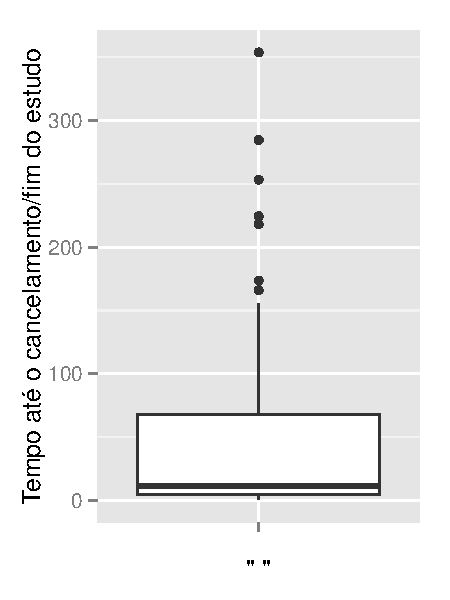
\includegraphics[width=\maxwidth]{figure/unnamed-chunk-4} 

\end{knitrout}
\caption{Boxplot do tempo até o cancelamento do cartão de crédito ou fim do acompanhamento}
\end{figure}

Na figura 3, vemos que os clientes em mediana têm o produto por 11 meses. Aproximadamente 75\% dos clientes tem tempo até 68 meses. O indivíduo que possui o produto a mais tempo, o tem a 353 meses. No estudo observamos que 18 clientes foram censurados, ou seja, ainda não tinham cancelado o cartão de crédito até a data de fim do acompanhamento.

Como não encontramos nenhuma irregularidade nas variáveis, passamos para uma análise descritiva bivariada. Aqui cruzamos as variáveis do banco de dados com o tempo até o cancelamento do produto, para assim termos dicas de como as variáveis estão relacionadas ao tempo que o cliente permanece com o cartão.


\begin{figure}[t!]

\centering
\begin{knitrout}
\definecolor{shadecolor}{rgb}{0.969, 0.969, 0.969}\color{fgcolor}
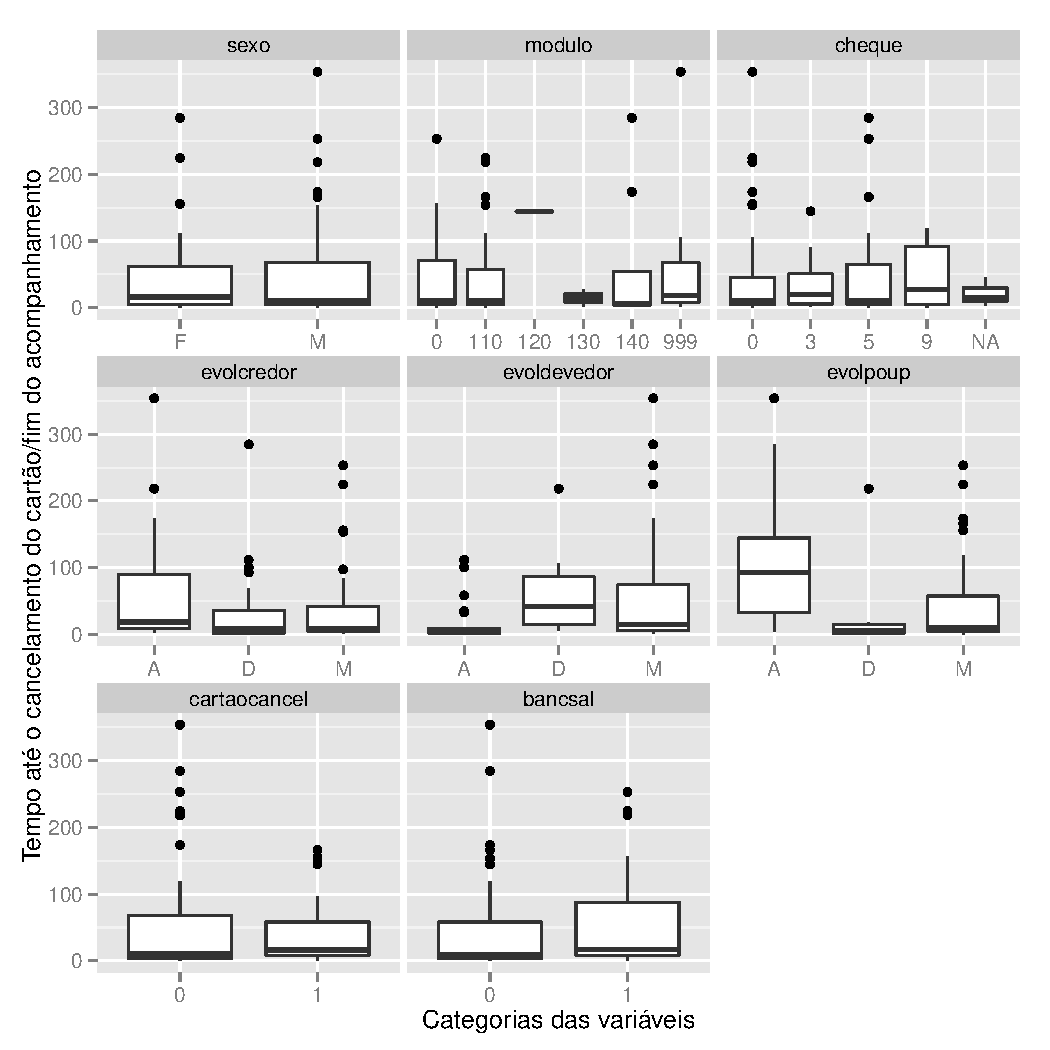
\includegraphics[width=\maxwidth]{figure/unnamed-chunk-5} 

\end{knitrout}
\caption{Curvas de sobrevivência estimadas por Kaplan-Meier para cada variável do banco de dados}
\end{figure}

Pelos gráficos da figura 5 podemos ver que não parece existir associação entre o sexo e o tempo, já que para as duas categorias as linhas se sobrepoem. O módulo também não parece influenciar, mas o tipo de conta e as evoluções de saldo devedor, creditor ou da poupança parecem apresentar diferenças no tempo até o cancelamento dependendo das categorias.
Os clientes que recebem o salário pelo banco tendem, aparentemente a ter tempos maiores.

\begin{figure}[t!]
\centering
\begin{knitrout}
\definecolor{shadecolor}{rgb}{0.969, 0.969, 0.969}\color{fgcolor}
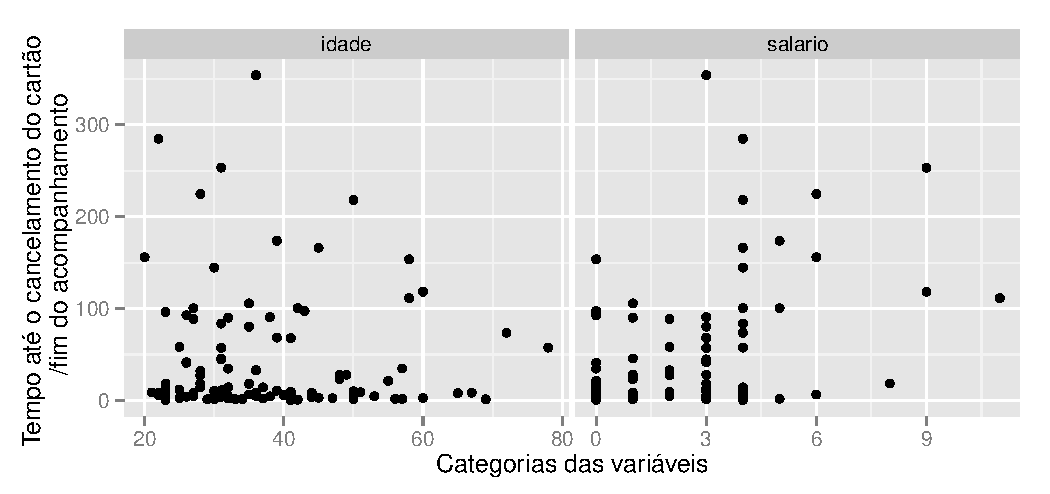
\includegraphics[width=\maxwidth]{figure/unnamed-chunk-6} 

\end{knitrout}
\caption{Gráficos de dispersão do tempo até o cancelamento do cartão/fim do acompanhamento pela idade e pela categoria de salário do cliente.}
\end{figure}

Nos gráficos da figura 6, é possível observar que o salário do cliente parece ser correlacionado positivamente com o tempo atée o cancelamento do cartão e que a idade não apresenta esse comportamento.

Após a análise descritiva, acreditamos que as principais variáveis para prever o tempo até o cancelamento do cartão são os saldos (credor, devedor e de poupança) e a categoria de salário do cliente. 

\section{Análise Inferencial}

Inicialmente vamos propor um modelo de Cox da forma:

$$\alpha(t|X) = \alpha_0(T)exp(t\beta)$$

Com $X$ um vetor com as covariáveis apresentadas na análise descritiva e $\beta$ os parâmetros associados a essas variáveis.
O ajuste do modelo foi feito no \texttt{R} usando o comando \texttt{coxph} do pacote \texttt{survival}. Já a seleção das variáveis explicativas foi feita usando o método `AIC`, isto é, selecionamos o modelo com o menor AIC. Como apenas três observações possuiam valores omisso em algumas das variáves, optamos por apenas excluí-las da análise. Optamos por não utilizar devido as duas variáveis "saldo credor" e "saldo devedor" juntas no modelo, pois por terem forte associação, a estimação dos parâmetros pode ser prejudicada. Por isso utilizamos apenas a variável evolcredor.


\begin{knitrout}
\definecolor{shadecolor}{rgb}{0.969, 0.969, 0.969}\color{fgcolor}\begin{kframe}
\begin{alltt}
\hlkwd{library}\hlstd{(survival)}
\hlstd{modelo} \hlkwb{<-} \hlkwd{coxph}\hlstd{(}\hlkwd{Surv}\hlstd{(tempo,status)} \hlopt{~} \hlstd{sexo} \hlopt{+} \hlstd{modulo} \hlopt{+} \hlkwd{as.factor}\hlstd{(cheque)} \hlopt{+} \hlstd{evolcredor} \hlopt{+}
                   \hlstd{evolpoup} \hlopt{+} \hlstd{idade} \hlopt{+} \hlstd{salario} \hlopt{+} \hlstd{cartaocancel} \hlopt{+} \hlstd{bancsal,}
                \hlkwc{data} \hlstd{=} \hlkwd{na.omit}\hlstd{(dados))}


\hlstd{modelo.a} \hlkwb{<-} \hlkwd{step}\hlstd{(modelo)}
\end{alltt}
\end{kframe}
\end{knitrout}

As variáveis explicativas selecionadas foram a evolução do saldo credor e da poupança além do salário e do indicador se o cliente recebe o salário pelo banco.
Todas as variáveis explicativas selecionadas pelo método AIC são significativas a nível de confiança 5\% pelo teste de Wald marginal.

Com o modelo escolhido, fizemos uma análise de diagnóstico para verificar a qualidade do ajuste. Analisamos o resíduo de Cox-Snell, que da uma ideia da qualidade geral do ajuste do modelo.

\begin{figure}[t!]
\centering
\begin{knitrout}
\definecolor{shadecolor}{rgb}{0.969, 0.969, 0.969}\color{fgcolor}
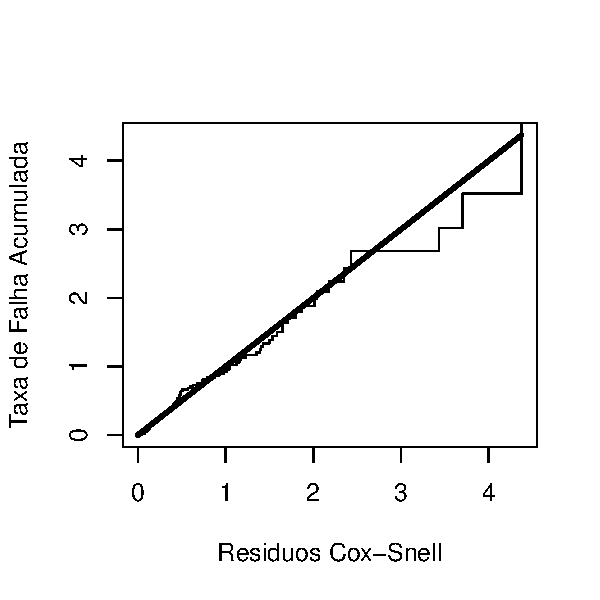
\includegraphics[width=\maxwidth]{figure/unnamed-chunk-8} 

\end{knitrout}
\caption{Gráfico da taxa de falha acumulada pelos resíduos de Cox-Snell, era esperado os pontos estivessem sobre/próximos a reta referência}
\end{figure}

O gráfico dos resíduos de Cox-Snell indicou que o ajuste geral do modelo parece ser adequado, já que os pontos estao próximos a reta referência. Não tendo problema com o ajuste geral do modelo, fizemos o gráfico do preditor linear pelo resíduo deviance, para assim poder identificar observações aberrantes que poderiam interferir nas estimativas do parâmetro.

\begin{figure}[t!]
\centering
\begin{knitrout}
\definecolor{shadecolor}{rgb}{0.969, 0.969, 0.969}\color{fgcolor}
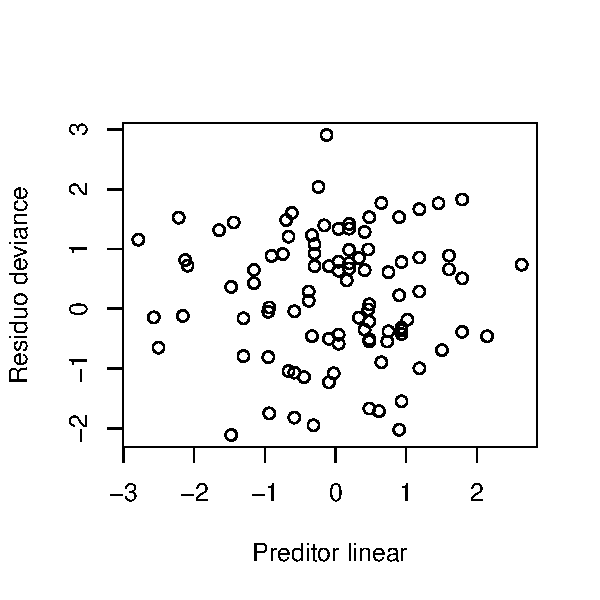
\includegraphics[width=\maxwidth]{figure/unnamed-chunk-9} 

\end{knitrout}
\caption{Gráfico do preditor linear pelo resíduo deviance. Esperamos que eles estejam distribuídos aleatoriamente e que não haja resíduos com valores em módulo maiores do que 2.}
\end{figure}

A partir da observação do gráfico podemos concluir que não existem pontos aberrantes. Além disso temos mais um indicativo de que o modelo de Cox está bem ajustado já que os valores dos resíduos estão aleatoriamente distribuidos de acordo com o preditor linear. Não observamos nenhum padrão, o que indicaria que o modelo não está bem ajustado.

A seguir apresentamos as estimativas dos parâmetros do modelo e discutiremos a interpretação dos resultados.

% latex table generated in R 3.1.0 by xtable 1.7-3 package
% Wed Nov 19 05:10:40 2014
\begin{table}[ht]
\centering
\begin{tabular}{rrrrrr}
  \hline
 & coef & exp(coef) & se(coef) & z & Pr($>$$|$z$|$) \\ 
  \hline
evolcredorD & 1.31 & 3.72 & 0.33 & 4.04 & 0.00 \\ 
  evolcredorM & 0.71 & 2.03 & 0.29 & 2.43 & 0.02 \\ 
  evolpoupD & 3.25 & 25.88 & 0.60 & 5.38 & 0.00 \\ 
  evolpoupM & 2.13 & 8.38 & 0.44 & 4.87 & 0.00 \\ 
  salario & -0.29 & 0.75 & 0.06 & -4.48 & 0.00 \\ 
  bancsal & -0.78 & 0.46 & 0.28 & -2.73 & 0.01 \\ 
   \hline
\end{tabular}
\caption{Estimativas dos parâmetros do modelo ajustado} 
\end{table}


Para facilitar a interpretação utilizaremos a tabela abaixo que apresenta as taxas de falha relativa estimadas bem como seus intervalos de confiança.

% latex table generated in R 3.1.0 by xtable 1.7-3 package
% Wed Nov 19 05:10:40 2014
\begin{table}[ht]
\centering
\begin{tabular}{rrrrr}
  \hline
 & exp(coef) & exp(-coef) & lower .95 & upper .95 \\ 
  \hline
evolcredorD & 3.72 & 0.27 & 1.97 & 7.04 \\ 
  evolcredorM & 2.03 & 0.49 & 1.15 & 3.60 \\ 
  evolpoupD & 25.88 & 0.04 & 7.92 & 84.63 \\ 
  evolpoupM & 8.38 & 0.12 & 3.56 & 19.69 \\ 
  salario & 0.75 & 1.33 & 0.66 & 0.85 \\ 
  bancsal & 0.46 & 2.17 & 0.26 & 0.80 \\ 
   \hline
\end{tabular}
\caption{Estimativas das razões de chance com base nos parâmetros do modelo ajustado} 
\end{table}


Utilizando as estimativas do modelo, podemos concluir que o fator mais importante para o cancelamento do cartão é a evolução do saldo da poupança. O cliente que diminui o saldo da poupança tem 24 vezes mais risco de cancelar do que um cliente como na referência (que aumentou o saldo credor, o saldo de poupança, não recebe o salário pelo banco e tem um salário baixo). O risco de cancelar quando o cliente manteve o saldo da poupança é 8 vezes o da referência.
O cliente que teve aumento no saldo devedor tem 3 vezes o risco de cancelar o cartão se comparado com a referência, já o que manteve o saldo tem 2 vezes esse risco.

Um fato interessante é o que o cliente que recebe o salário pelo banco tem 2 vezes menos risco de cancelar o cartão quando comparado a referência. Quanto maior o salário, menor o risco de cancelamento também, a cada aproximadamente 500 reais o risco diminui cerca de 30\%.

\nocite{sobrev}
\bibliographystyle{unsrt}%Used BibTeX style is unsrt
\bibliography{bibliografia}









\end{document}
